\documentclass[aspectratio=169]{beamer}

%\setbeameroption{show only notes}

\usepackage[utf8]{inputenc}
\usepackage{hyperref}
\usepackage{booktabs}
\usepackage{csquotes}
\usepackage[style=authoryear,backend=biber]{biblatex}
\addbibresource{nlp-for-ch/01-Semantics.bib}
\addbibresource{nlp-for-ch/02-Machine-Translation.bib}

\addtolength{\skip\footins}{4pc plus 8pt}

% Questo tema commentato di sotto produce un beamer più tradizionale 
%\usetheme[secheader]{Boadilla}


%%%-----------------------------------------------------------%
%% Cambia colori da thema default
%% Questi sono i due colori ufficiali rosso e grigio
\definecolor {cfred}{rgb}{0.709,0.196,0.329} 	%{ 181 ,50 ,84}
\definecolor {cfgrey}{rgb}{0.537,0.537,0.537} 	%{ 137,137,137}
\definecolor {cflink}{rgb}{0.615,0.615,0.607} 	%{157,157,155}

\setbeamercolor{palette primary}{bg=cfred,fg=white}
\setbeamercolor{palette secondary}{bg=cfred,fg=white}
\setbeamercolor{palette tertiary}{bg=cfred,fg=white}
\setbeamercolor{palette quaternary}{bg=cfred,fg=white}
\setbeamercolor{structure}{fg=cfred}		 % itemize, enumerate, etc
\setbeamercolor{section in toc}{fg=cfred} 		 % TOC sections
% Override palette coloring with secondary
\setbeamercolor{subsection in head/foot}{bg=cfgrey,fg=white}
%%%------------------------------------------------------------

%% Definisce il blocco con riquadro che non è presente nel tema default (commentare se si usano altri temi)
\setbeamercolor{uppercolor}{fg=white,bg=cfred}%
\setbeamercolor{lowercolor}{fg=black,bg=white}%
\def \bblock{\begin{beamerboxesrounded}[upper=uppercolor,lower=lowercolor,shadow=true]}
\def \eblock{\end{beamerboxesrounded}}

\defbeamertemplate{description item}{align left}{\insertdescriptionitem\hfill}
\setbeamertemplate{description item}[align left]
%%-----------------------------------------------------------

%% Intestazione ripetuta per ogni slide
\addtobeamertemplate{headline}{%
    \vspace{0.25cm} \ \ 
    
\includegraphics[height=1.0cm]{images/fedhlab4.png} 	% sostituire con logobeamIT.png per italiano
    \hspace{0.541\textwidth}{\color{cflink} {\small NLP4CH}} %per 16:9 641 for link
    %\hspace{0.551\textwidth}{\color{cflink} {\small www.unive.it}} %per 4::3
    \vspace{0.25cm}
    {\color{cfred} \hrule \hrule  }
    \textbf{}
}{}
\setbeamertemplate{footline}[text line]{%
  \parbox{\linewidth}{\vspace*{-8pt}%
  {\color{cflink} {%
  Page \insertpagenumber/\inserttotalframenumber~--  CC-BY 4.0 -- thibault.clerice@inria.fr
}}}}

\setbeamertemplate{page number in head/foot}[appendixframenumber]
%%-------------------------------------------------------------

%This block of code defines the information to appear in the Title page
%%%
\title[NLP 4 CH] %optional
{Semantics in Natural Language Processing}

\author[Clérice, Thibault] % (optional)
{T.~Clérice~\inst{1}~\inst{2}}

\institute[Inria] % (optional)
{
  \inst{1}%
  ALMAnaCH, Inria, Paris, France \and
  \inst{2}%
  FeDHLab, Università Federico II, Napoli, Italia
 }

\date[2024] % (optional)
{Natural Language Processing for CH}

\setbeamertemplate{frametitle}[default][right, rightskip=.5cm] {}
\addtobeamertemplate{frametitle}{\vspace*{-1.4cm}}{}
%End of title page configuration block
%------------------------------------------------------------


%------------------------------------------------------------
%The next block of commands puts the table of contents at the 
%beginning of each section and highlights the current section:

\AtBeginSection[]
{
  \begin{frame}
    \frametitle{Table of Contents}
    \tableofcontents[currentsection]
  \end{frame}
}
%------------------------------------------------------------

\setbeamerfont{footnote}{size=\tiny} %reduce the size of the footnote citation

\addtobeamertemplate{footnote}{}{\vspace{2.2ex}}
\begin{document}

%The next statement creates the title page.
\frame{\titlepage}

\begin{frame}{The course}
    \begin{enumerate}
        \item (Today) Semantics in Natural Language Processing;
        \item Machine Translation;
        \item Annotating text: lemmatization, POS tagging, abbreviation resolution ?
        \item (Hands-on) Producing a corpus
        \item (Hands-on) Producing a corpus
        \item (Hands-on) Producing a corpus and seeing the results
    \end{enumerate}
\end{frame}

\section{Introduction}

\begin{frame}{Founding Hypothesis}
    The founding elements for computational semantics is the \textbf{distributional hypothesis}. It is often attributed to John Rupert Firth, specifically through this quote from 1957: ``You shall know a word by the company it keeps''\footfullcite{firth1957synopsis}.
    \vspace{1em}
    This statement can be exemplified by a ``fill-the-word'' sentence such as "This morning, I drank a an orange \textit{BLANK}'' or ``At \textit{BLANK}, during recess, I played cards''.
\end{frame}

\begin{frame}{Approaches of this hypothesis}
    Based on the computation power, the research advances in other areas and the size of corpora, this hypothesis has known various computational implementations:
    \begin{itemize}
        \item Co-occurrences Matrixes
        \item Word Embeddings (Word2Vec and Fasttext)
        \item Contextual Embeddings
    \end{itemize}
\end{frame}

\begin{frame}{Similarity and vectors}
    In any case, words are represented as vectors. A vector is a series of value, of a given length, generally noted such as $V_{\text{dog}} = [.4, .3, .2, .1 ...] $ and $V_{\text{cat}} = [.4, .3, .2, .1 ...] $. A vector can be thought as the representation in N-dimensions of a word, such that in the same space, two words will be "geographically" close to each others. Cosine distance are the most preferred way to compute this similarity.

    Similarity is not synonymy ! Similarity is a mix of semantic and syntactic connections between two terms: two antonyms (hate and love) will be much closer than two words mostly unrelated to each other (hate and broccoli).
\end{frame}

\begin{frame}{Example}
    \centering
    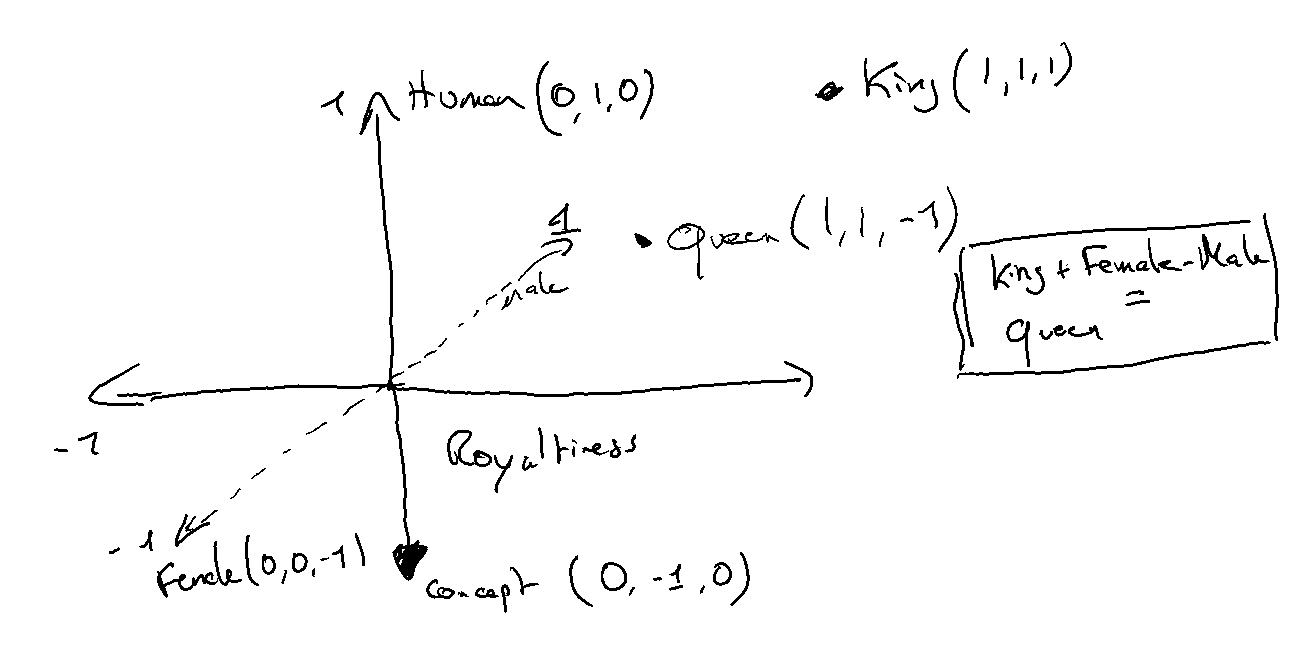
\includegraphics[width=.9\linewidth]{nlp-for-ch/images/vectors.png}
\end{frame}

\section{Co-occurrences Matrices}

\begin{frame}{How ?}
    \centering
    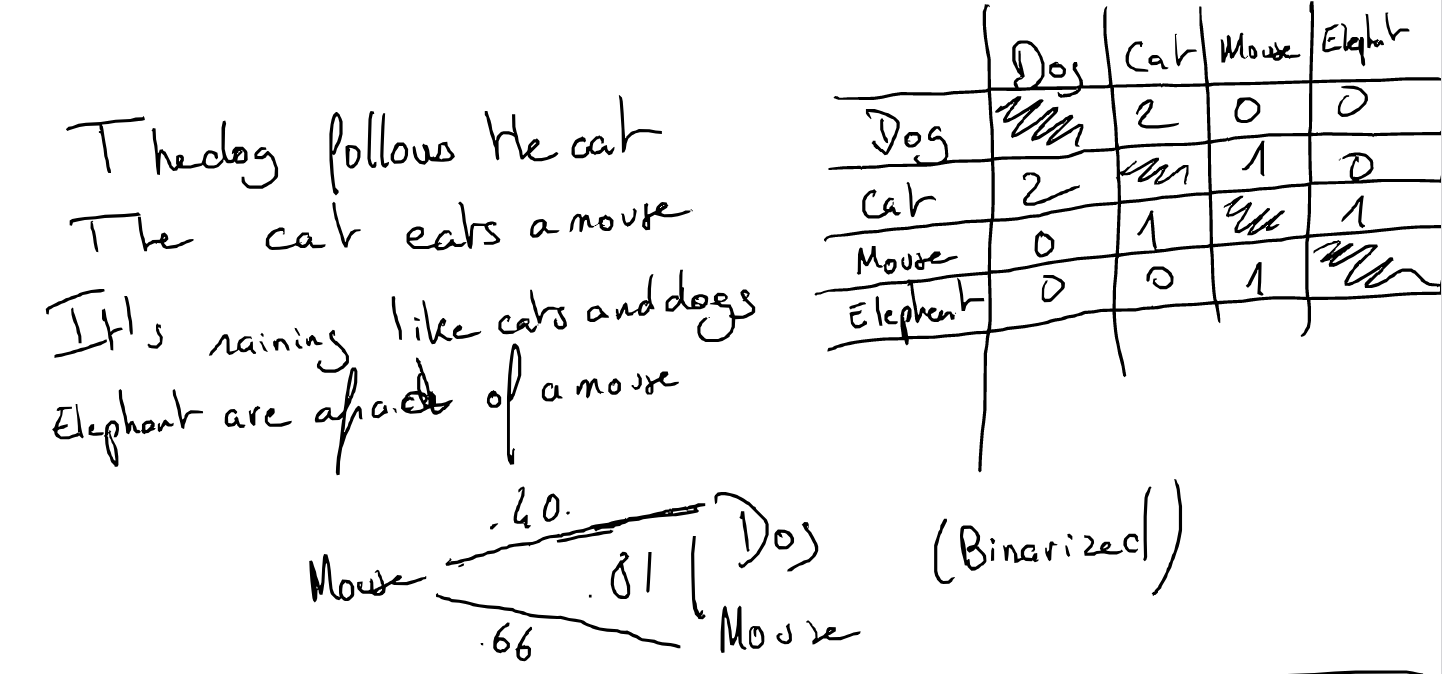
\includegraphics[width=.9\linewidth]{nlp-for-ch/images/cooccmatrices.png}
\end{frame}


\begin{frame}{Counting co-occurrences}
    Generally one parameter which is the \textit{window size}: how far in a sentence can we say that two words are related. This window size can be dependent on the language or the corpus in general.
    
    The co-occurrence matrix has seen various way to be designed:
    \begin{itemize}
        \item Word count;
        \item Relative Frequency;
        \item Binarized (Presence / Absence);
        \item Proximity weighting
    \end{itemize}
\end{frame}

\begin{frame}{And Simplification ?}
    And it can then be simplified again, specifically with a reduction of the parameters such as Principal Component Analysis, Singular Value Decomposition, etc. This is especially important in the context of large corpus. If you have 4 million of words, and 10~000 unique word forms, your co-occurrence matrix will be 10~000 by 10~000, which makes any computation heavy. 

    PCA, SVD and other approaches then reduce this by finding similarity in the data in a compute efficient way, so that the original 10~000 columns of co-occurrences become a few 100. These columns do not represent words anymore but starts to represent abstract traits (syntactic or semantic).

    Then, with smaller vector, distances at scale is easier to compute !
\end{frame}

\section{Word2Vec and FastText}

\begin{frame}{The limits of co-occurrences as a matrix}
    \begin{itemize}
        \item VERY heavy for a very large corpus
        \item Is relatively limited when it comes to reduction (nobody wants a vocabulary of size 130000 and vectors of size 130000) efficiency.
    \end{itemize}
    Solutions ? Machine learning:
    \begin{itemize}
        \item \fullcite{mikolov2013distributed}
    \end{itemize}
\end{frame}

\begin{frame}{Mikolov's improvements}
    \centering
    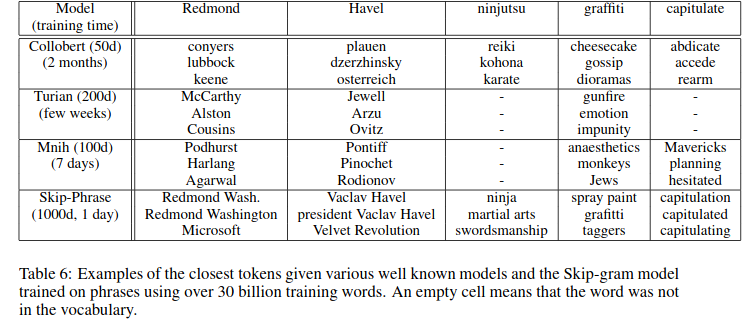
\includegraphics[width=.9\linewidth]{nlp-for-ch/images/mikolov.png}
\end{frame}


\begin{frame}{How does it work ?}
    \centering
    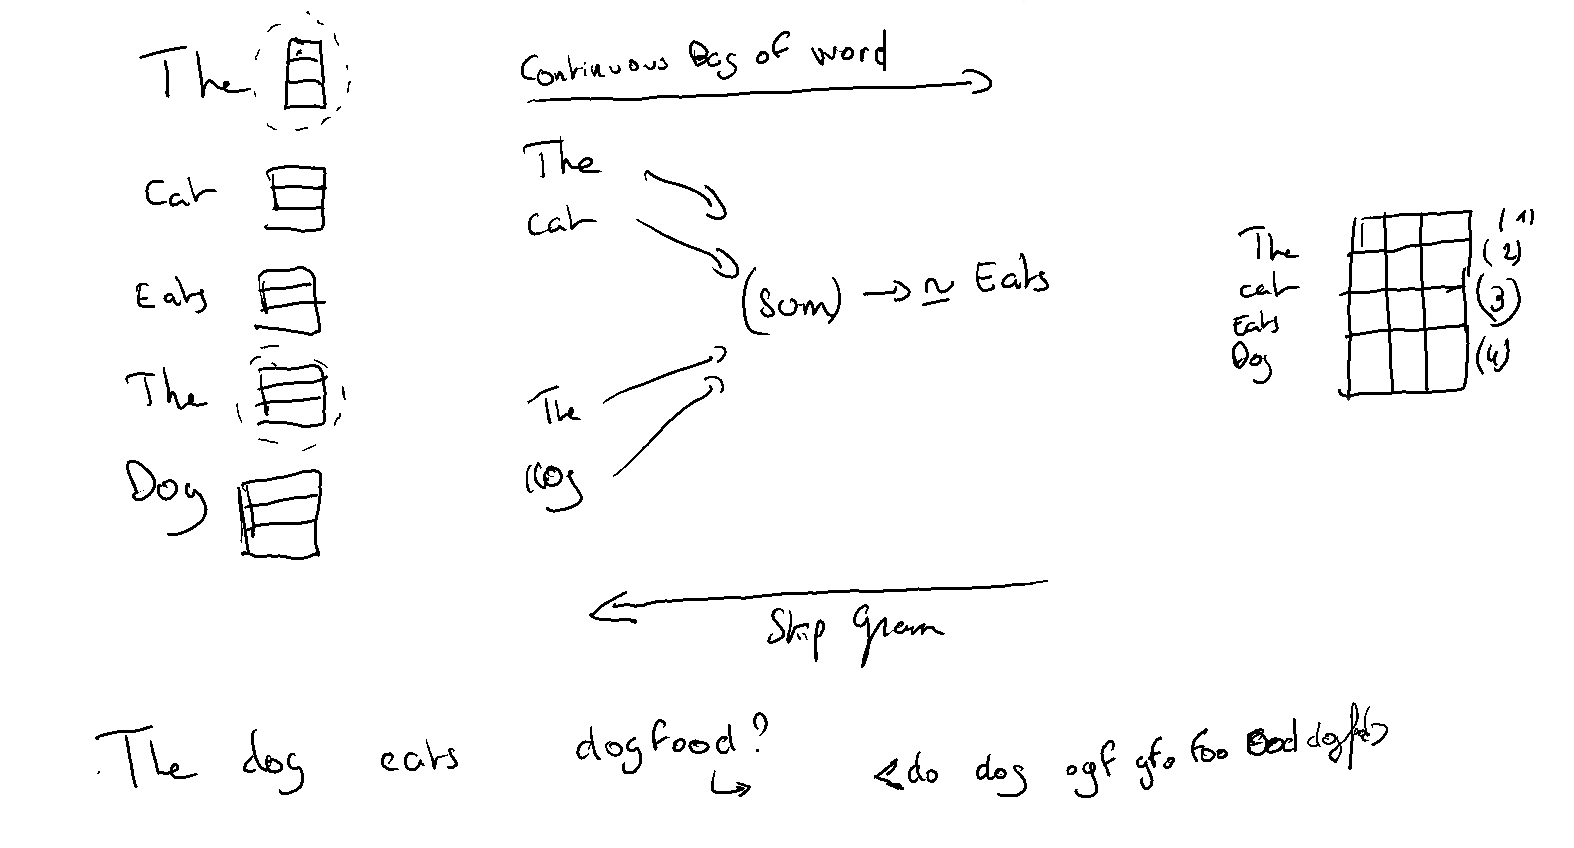
\includegraphics[width=.8\linewidth]{nlp-for-ch/images/word2vec.png}
\end{frame}

\begin{frame}{Variability ?}
    \begin{columns}
        \begin{column}{.4\linewidth}
            Measuring stability across three experiments settings: (Fixed Order [ABC, ABC, ABC], shuffled order [ACB, BAC, CBA], repetition [BAA, CAB, BBB]) for different size of corpora of globally coherent domains (in one language): 2.6 M, 4.2 M, 6.2 M, 12.2 M, 14.6 M, 20.5 M tokens.
        \end{column}
        \begin{column}{.6\linewidth}
        \begin{itemize}
            \item ``In general, LSA, GloVe, SGNS, and PPMI are not sensitive to document order. [...] All four algorithms are sensitive to the presence of specific documents, though this effect is weaker for PPMI.''
            \item ``We emphasize that with smaller corpora comes greater variability [...] The size of the corpus, the length of individual documents, and the presence or absence of specific documents can all affect the resulting embeddings''
        \end{itemize}
        \end{column}
    \end{columns}
    \vspace{1em}
    {\small \fullcite{antoniak2018evaluating}}
\end{frame}

\section{Bert}

\begin{frame}{Again, dealing with limitations !}
    \begin{itemize}
        \item Word2Vec and Fasttext are nice... But words sense are not contextual : they are global !
        \item Very bad for polysemy;
        \item Very bad for large vocabulary;
        \item Potentially bad for bad words.
    \end{itemize}
    New limitations:
    \begin{itemize}
        \item Compute is HUGE;
        \item Data needs to be huge.
    \end{itemize}
\end{frame}

\begin{frame}{How does it work ?}
    \centering
    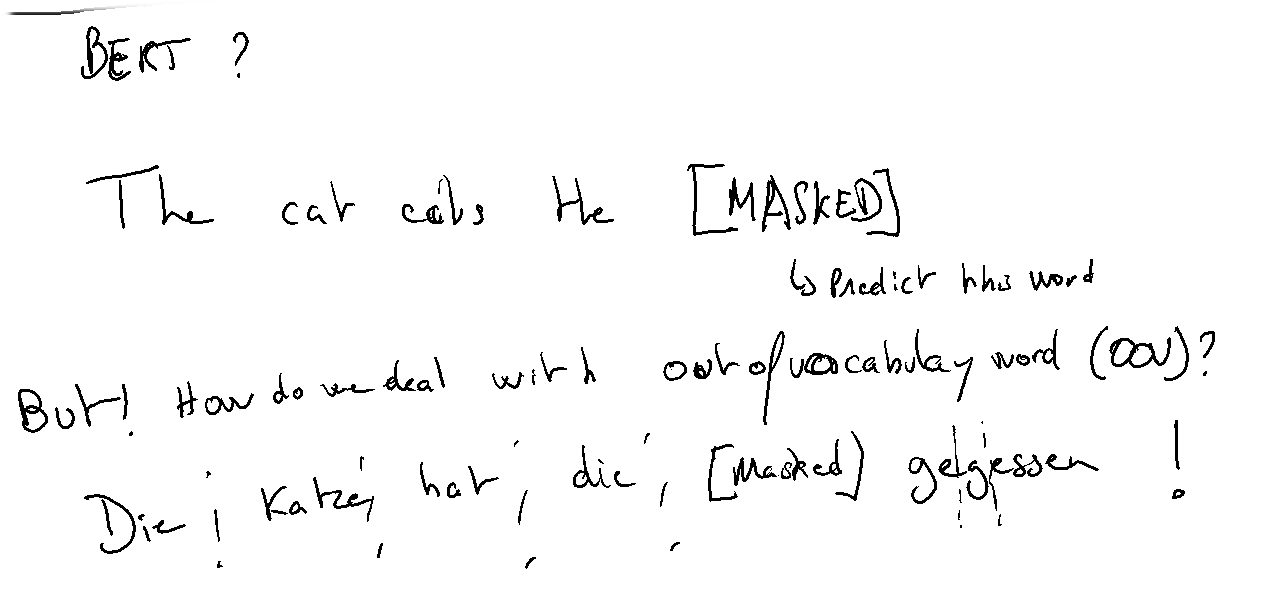
\includegraphics[width=.9\linewidth]{nlp-for-ch/images/bert.png}
\end{frame}

\section{Pedrazzini \& Mc Gillivray, 2022}

\begin{frame}{Paper}
    \fullcite{pedrazzini-mcgillivray-2022-machines}
    \vspace{1em}
    
    \small \textbf{Abstract:} ``The industrialization process associated with the so-called Industrial Revolution in 19th-century Great Britain was a time of profound changes, including in the English lexicon. An important yet understudied phenomenon is the semantic shift in the lexicon of mechanisation. In this paper we present the first large-scale analysis of terms related to mechanization over the course of the 19th century in English. We draw on a corpus of historical British newspapers comprising 4.6 billion tokens and train historical word embedding models. We test existing semantic change detection techniques and analyse the results in light of previous historical linguistic scholarship''
\end{frame}

\begin{frame}{An alternative approach to Denove et al.}
    \begin{itemize}
        \item A relatively similar question and corpus to Denove et al.: does the mechanization and the industrial revolution affects discourses and how fast ?
        \item Few differences though: unilingual, focus on semantic shifts (word2word) rather than topic shift (word-topic-topic-word).
        \begin{itemize}
            \item This also eliminates any human interpretation of topic labelling, and as such is stronger.
            \item Embeddings are computed at the sentence level, which mitigates the issues of articles not being recognized as such through the Bag of words approach of topic modelling (which does not work with co-occurrence in a small window but in the document).
        \end{itemize}
    \end{itemize}
\end{frame}

\begin{frame}{Method}
    \begin{itemize}
        \item Two newspaper collections: 119 newspaper titles, 1801-1920, 4.5 billion tokens.
        \item The number of titles should impact the result by normalizing political leaning and regional differences, even in the English language.
        \item Removal of stopwords, preprocessing of the text. Data at the articles level thanks to the Living with Machines and Heritage Made Digital projects.
        \item Hyperparameters chosen on a single decade, and applied the same way through the corpus.
        \item Alignments of the semantic spaces using Orthogonal Procrustes (I'll pass on the maths)
        \item Detection of Significant Changepoints
    \end{itemize}
\end{frame}

\begin{frame}{Three Results}
    \begin{columns}[c]
        \begin{column}{.50\linewidth}
            {\small
            \begin{itemize}
                \item<1-> \textbf{Train} clearly changes sense from ‘an elongated back of a robe or skirt’ to ‘a
    series of connected railway carriages’.
                \item<2-> \textbf{Wheel} does not change sense \textit{per se}, but its context shifts and represent new usages: paddle wheel (mississipi boat wheels), steering wheels, etc. We see a mechanization contextual shift.
                \item<3> \textbf{Fellow} basically gets a new kind of usage or at least the reinforcement of a non academic usage, such as fellow countrymen, fellow citizens, which is used as an address in political discourses (maybe more and more as the reading capable citizen gets the ability to read)
            \end{itemize}
            }
        \end{column}
        \hfill
        \begin{column}{.45\linewidth}
            \centering
            \includegraphics<1>[width=\linewidth]{nlp-for-ch/images/train.png}
            \includegraphics<2>[width=\linewidth]{nlp-for-ch/images/wheel.png}
            \includegraphics<3>[width=\linewidth]{nlp-for-ch/images/fellow.png}
        \end{column}
    \end{columns}
\end{frame}

\begin{frame}{Quality Control and Limitations}
    \begin{itemize}
        \item Hyperparameters tested through an analysis of potential change points for words that would be semantically stable and synonyms through the 19th-century
        \item Many back and forth between quantiative and qualitative studies (\textit{A history of the English Language in the Nineteenth Century} by Görlach (1999) and in general the Oxford English Dictionary for the recorded apparition of senses))
    \end{itemize}
\end{frame}

\section{Clérice, 2024}

\begin{frame}{Paper}
    \fullcite{clerice2024detecting}
    
    \fullcite{cleri2022}
    
    \vspace{1em}
   \textbf{Question:} How does one detect sentences with sexual meaning in Latin in diachrony?
\end{frame}

\begin{frame}{Corpus}
    \begin{itemize}
        \item Drew examples from James N.~Adams' ``Latin Sexual Vocabulary'' (1982).
        \begin{itemize}
            \item Definition of sexuality quite restrictive (mostly the act itself, virginity is out of the picture, same for fore-foreplay).
            \item But Adams does have large (but quite uneven) chronological coverage
        \end{itemize}
        \item Train a model that would creates embeddings of sentences, and see if it could identify as bearing sexual semantics.
        \begin{itemize}
            \item Optionally telling us which word(s) are bearing the load.
        \end{itemize}
    \end{itemize}
\end{frame}

\begin{frame}{Four levels of difficulty}
   \begin{itemize}
        \item specific lexemes within the semantic field, e.g. ``Quid faciat uolt scire Lyris. Quod sobria: fellat.\footnote{``Lyris wants to know what she does [drunk]. What she does sober: she sucks (\textit{fellat}).''}'', Martial, \textit{Epigrammata}, II, 73. 
        \item lexemes used metaphorically within the field, e.g. ``Tanta est quae Titio columna pendet , Quantam Lampsaciae colunt puellae.\footnote{``The column (\textit{columna}) that hangs from Titius is so large that the young girls of Lampsaka venerate it.''}'', Martial, \textit{Epigrammata}, XI, 51.
        \item complex and unique figurative speech, e.g. ``Donec proterua nil mei manu carpes, licebit ipsa sis pudicior Vesta.\footnote{``As long as you don't pick anything from me with a shameless hand, you'll be chaster than Vesta herself.'' (Implying that if someone steals something from Priapus, who is talking here, they will be sexually assaulted).}'',  Anonymous, \textit{Priapea}, 31.
        \item Graphic pun (such as CD) or sound-based reference (``illam dicam'' = 'landica', ``cum nos'' = cunnus, cf. Cicero) which are probably the most difficult.
    \end{itemize}
\end{frame}

\begin{frame}{Method}
    \begin{itemize}
        \item Evaluate multiple methods, train on various size of the corpus
        \item Compare with plain text search
        \item Evaluate reusability of the method
    \end{itemize}
\end{frame}

\begin{frame}{Network}
    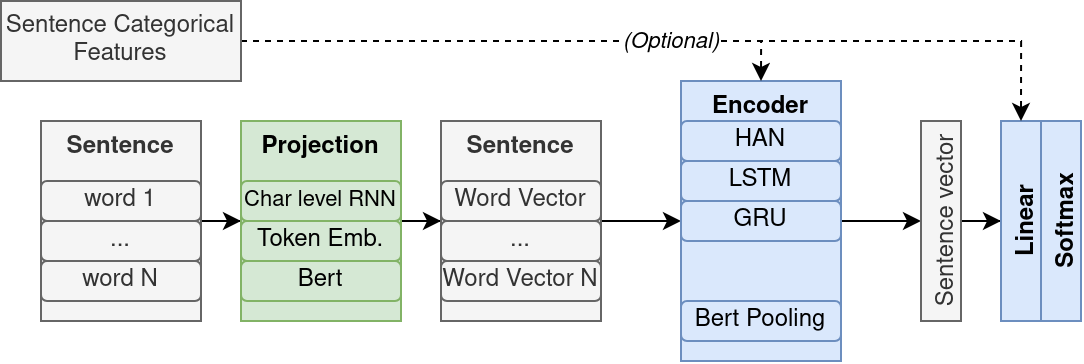
\includegraphics[width=\linewidth]{nlp-for-ch/images/layers.png}
\end{frame}

\begin{frame}{Results}
    \begin{table}[ht]
    \resizebox{\linewidth}{!}{%}
    \begin{tabular}{llllll}
    \hline
    {} & & TPR & TNR &   Precision &          F1 \\
    Embedding & Model             &                   &                   &             &             \\ \hline
     & Baseline 1 & 100.0 & 7.43 & 9.82 & 17.88  \\
     & Baseline 2 & 100.0 & 12.32 & 10.31 & 18.69  \\
     & Baseline 3 & 98.8 & 48.37 & 16.17 & 27.79  \\
     & Baseline 4 & 74.9 & 72.34 & 21.44 & 33.34  \\
    \hline
    Lemma & GRU-256           &        65.78 ± 5.82 &        \textbf{98.92 ± 0.64} &  \textbf{86.65 ± 5.13} &  74.45 ± 2.59 \\
    Lemma & HAN-256           &        \textbf{70.60 ± 2.83} &        98.76 ± 0.30 &  85.33 ± 2.75 &  \textbf{77.20 ± 1.35} \\
    Token & HAN-128           &        57.81 ± 5.37 &        98.82 ± 0.42 &  83.51 ± 3.79 &  68.06 ± 3.11 \\
    Token & GRU-128           &        59.16 ± 5.37 &        98.74 ± 0.35 &  82.81 ± 3.37 &  68.81 ± 3.16 \\
    Token & LSTM-128          &        57.01 ± 3.11 &        98.76 ± 0.26 &  82.33 ± 2.52 &  67.29 ± 1.84 \\
    \hline
    \end{tabular}
    }
    \caption{Median scores over 10 trained models for each model per embedding and encoder. ``Lemma'' or ``token'' stand for the concatenation of word level embedding and character level embeddings of the given input.}
    \label{tab:main-scores}
    \end{table}
\end{frame}

\begin{frame}{Qualitative result}
    \begin{itemize}
        \item Some metaphors require real world knowledge, such as geographical features that reminds the reader of an anus in the sea (an epigram of Ausonius).
        \item Some polysemic words get sometime caught in the middle, such as \textit{uterus}, but this could potentially be fixed by adding more true negative with uterus in other senses.
        \item Able to pick-up on interesting complex structures: ``Donec proterua nil mei manu carpes ,
licebit ipsa sis pudicior Vesta.'' (As long as you do not pick anything from my garden with a brazen hand, You can be purer than Vesta herself.). or  ``Nox tibi, si belles, possit, Homere, dari.'' (If you had been fighting in the war, Homer, night(s) could have been given to you.'').
        \item Able to provide information about the choice (most important words)
    \end{itemize}
\end{frame}

\section{Next week's papers}

\begin{frame}{Next week}
    \small Presentation by S.~Gabay of his work on Machine Translation applied to the Humanities.
    {\footnotesize
    \begin{itemize}
        \item \fullcite{bawden-etal-2022-automatic}
        \item \fullcite{gabay2022vers}
        \item \fullcite{gabay2022ancien}
        \item \fullcite{gabay2024reconnaissance}
        \item \fullcite{gabay:hal-04704549}
    \end{itemize}
    }
\end{frame}

\end{document}